\documentclass[tikz,border=10pt]{standalone}

\usepackage{tikz}

\begin{document}

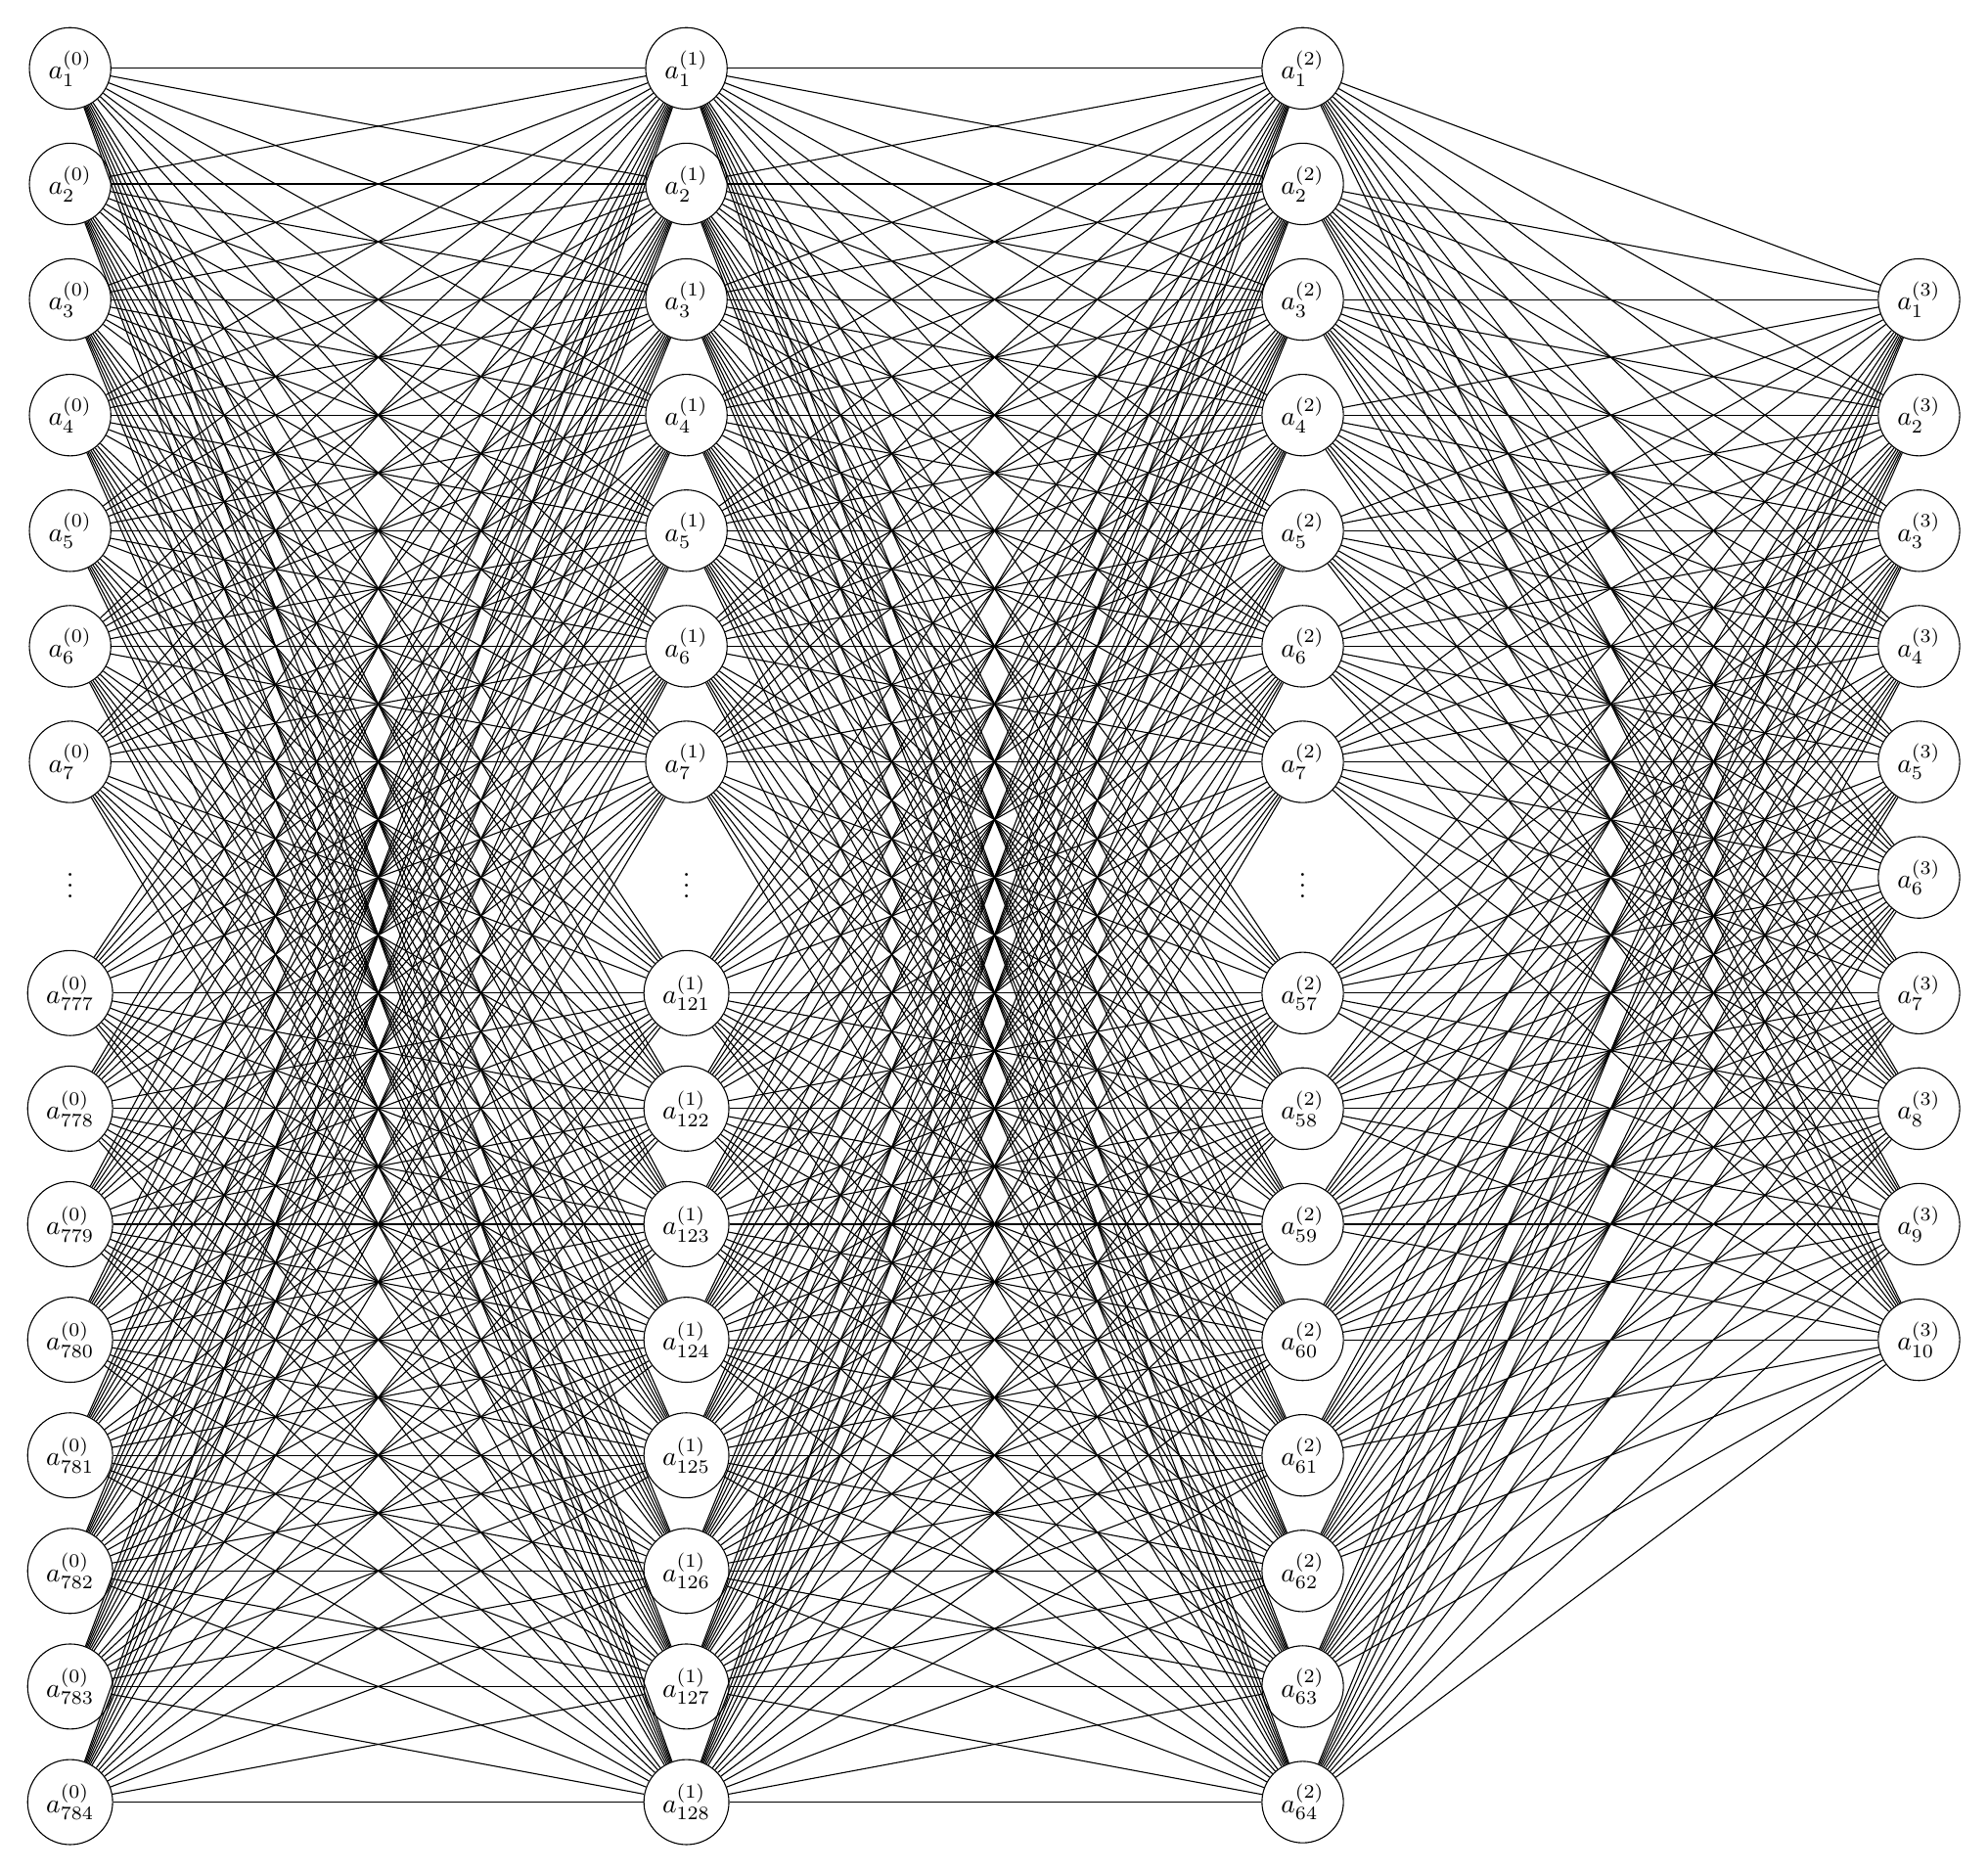
\begin{tikzpicture}[
    neuron/.style={circle, draw, minimum size=1cm}
]

    % 128 64 10

    \foreach \i in {1,...,7}
        \node[neuron] (I\i) at (0,-{\i}*1.5) {$a_{\i}^{(0)}$};

    \node at (0, {-8*1.5}) {\vdots};

    \foreach \i [evaluate=\i as \k using int(784-15+\i)] in {8,...,15}
        \node[neuron] (I\i) at (0,-{\i}*1.5-1.5) {$a_{\k}^{(0)}$};

    % First hidden layer
    \foreach \i in {1,...,7}
        \node[neuron] (H1\i) at (8,-{\i}*1.5) {$a_{\i}^{(1)}$};

    \node at (8, {-8*1.5}) {\vdots};

    \foreach \i [evaluate=\i as \k using int(128-15+\i)] in {8,...,15}
        \node[neuron] (H1\i) at (8,-{\i}*1.5-1.5) {$a_{\k}^{(1)}$};

    % Second hidden layer
    \foreach \i in {1,...,7}
        \node[neuron] (H2\i) at (16,-{\i}*1.5) {$a_{\i}^{(2)}$};

    \node at (16, {-8*1.5}) {\vdots};

    \foreach \i [evaluate=\i as \k using int(64-15+\i)] in {8,...,15}
        \node[neuron] (H2\i) at (16,-{\i}*1.5-1.5) {$a_{\k}^{(2)}$};


    % Output layer
    \foreach \i in {1,...,10}
        \node[neuron] (O\i) at (24,-{\i}*1.5-3) {$a_{\i}^{(3)}$};

    % Connections

    \foreach \i in {1,...,15}
        \foreach \j in {1,...,15}
            \draw (I\i) -- (H1\j);

    \foreach \i in {1,...,15}
        \foreach \j in {1,...,15}
            \draw (H1\i) -- (H2\j);

    \foreach \i in {1,...,15}
        \foreach \j in {1,...,10}
            \draw (H2\i) -- (O\j);


\end{tikzpicture}

\end{document}
